\documentclass[a4paper, 12pt]{article}
\usepackage[english]{babel} % or \usepackage[vietnamese]{babel}
\usepackage[utf8x]{inputenc}
\usepackage{amsmath, graphicx, tikz}
\usetikzlibrary{calc}
\usepackage[utf8]{vietnam}
\usepackage{subfigure}
\usepackage{gensymb}
%\usepackage{mathptmx}
\setlength{\parindent}{0pt}
\begin{document}

\begin{titlepage}
	
\begin{tikzpicture}[remember picture,overlay,inner sep=0,outer sep=0]
\draw[blue!70!black,line width=4pt] ([xshift=-1.5cm,yshift=-2cm]current page.north east) coordinate (A)--([xshift=1.5cm,yshift=-2cm]current page.north west) coordinate(B)--([xshift=1.5cm,yshift=2cm]current page.south west) coordinate (C)--([xshift=-1.5cm,yshift=2cm]current page.south east) coordinate(D)--cycle;

\draw ([yshift=0.5cm,xshift=-0.5cm]A)-- ([yshift=0.5cm,xshift=0.5cm]B)--
([yshift=-0.5cm,xshift=0.5cm]B) --([yshift=-0.5cm,xshift=-0.5cm]B)--([yshift=0.5cm,xshift=-0.5cm]C)--([yshift=0.5cm,xshift=0.5cm]C)--([yshift=-0.5cm,xshift=0.5cm]C)-- ([yshift=-0.5cm,xshift=-0.5cm]D)--([yshift=0.5cm,xshift=-0.5cm]D)--([yshift=0.5cm,xshift=0.5cm]D)--([yshift=-0.5cm,xshift=0.5cm]A)--([yshift=-0.5cm,xshift=-0.5cm]A)--([yshift=0.5cm,xshift=-0.5cm]A);

\draw ([yshift=-0.3cm,xshift=0.3cm]A)-- ([yshift=-0.3cm,xshift=-0.3cm]B)--
([yshift=0.3cm,xshift=-0.3cm]B) --([yshift=0.3cm,xshift=0.3cm]B)--([yshift=-0.3cm,xshift=0.3cm]C)--([yshift=-0.3cm,xshift=-0.3cm]C)--([yshift=0.3cm,xshift=-0.3cm]C)-- ([yshift=0.3cm,xshift=0.3cm]D)--([yshift=-0.3cm,xshift=0.3cm]D)--([yshift=-0.3cm,xshift=-0.3cm]D)--([yshift=0.3cm,xshift=-0.3cm]A)--([yshift=0.3cm,xshift=0.3cm]A)--([yshift=-0.3cm,xshift=0.3cm]A);

\end{tikzpicture}

\newcommand{\HRule}{\rule{\linewidth}{0.5mm}} % Defines a new command for the horizontal lines, change thickness here

\centering % Center everything on the page
 
%	HEADING SECTIONS
\textsc{\LARGE ĐẠI HỌC BÁCH KHOA TP. HCM}\\[1cm] % Name of your university/college
\textsc{\Large KHOA ĐIỆN ĐIỆN TỬ}\\[0.5cm] % Major heading such as course name
\textsc{\large BỘ MÔN TỰ ĐỘNG}\\[0.5cm] % Minor heading such as course title

%	TITLE SECTION
\HRule \\[0.4cm]
{ \huge \bfseries ĐỀ CƯƠNG TỐT NGHIỆP }\\[0.4cm] % Title of your document
\HRule \\[1cm]
 
%	AUTHOR SECTION
\begin{minipage}{0.4\textwidth}
\begin{flushleft} \large
\emph{Sinh viên:}\\
\textsc{Tạ Minh Đức} \\% Your name
\textsc{MSSV: 1510812}\\
\textsc{Huỳnh Nhật Tú} \\% Your name
\textsc{MSSV: }
 
\end{flushleft}
\end{minipage}
~
\begin{minipage}{0.4\textwidth}
\begin{flushright} \large
\emph{GVHD:} \\
\textsc{Nguyễn Vĩnh Hảo} % Supervisor's Name
\end{flushright}
\end{minipage}\\[1cm]

% If you don't want a supervisor, uncomment the two lines below and remove the section above
%\Large \emph{Author:}\\
%Vu \textsc{Hong Quan}\\[3cm] % Your name

%	LOGO SECTION

\includegraphics[scale=0.25]{images/LogoBK.jpg}\\[1cm] % Include a department/university logo - this will require the graphicx package

%	DATE SECTION
{\large \today}\\[0cm] % Date, change the \today to a set date if you want to be precise

\vfill % Fill the rest of the page with whitespace
\end{titlepage}

\tableofcontents
\begin{abstract}
Your abstract.
\end{abstract}
\section{Phần cứng}
\subsection{Các module sử dụng}
\begin{figure}[h]%
	\centering
	\subfigure[Power.]{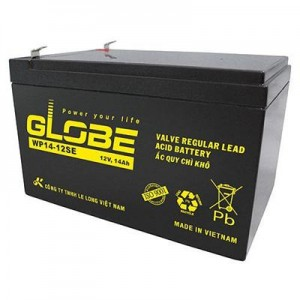
\includegraphics[width=.3\linewidth]{images/power.jpg}}\qquad
	\subfigure[Driver.]{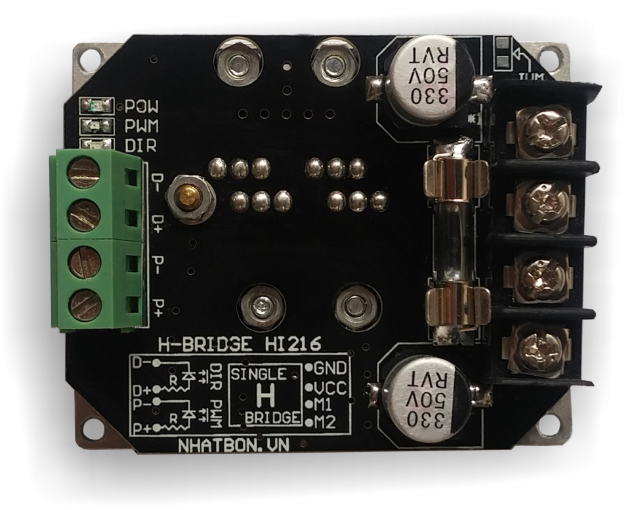
\includegraphics[width=.3\linewidth]{images/driver.png}}\qquad
	\subfigure[STM32F411.]{\label{3figs-c}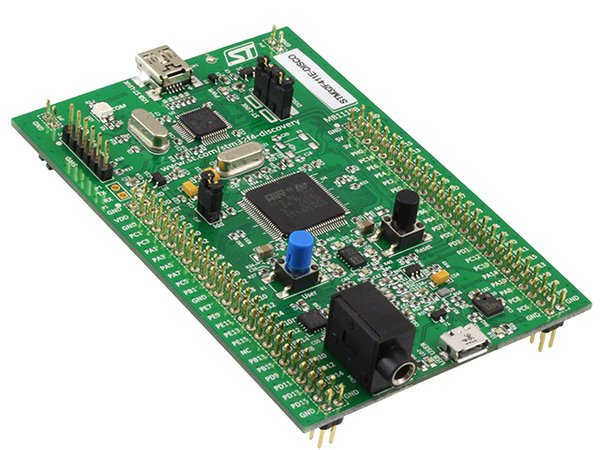
\includegraphics[width=.3\linewidth]{images/stm32f4.jpg}}\quad
	\subfigure[LORA.]{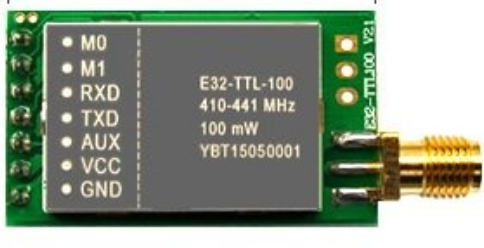
\includegraphics[width=.3\linewidth]{images/lora.png}}\quad
	\subfigure[RTK GPS.]{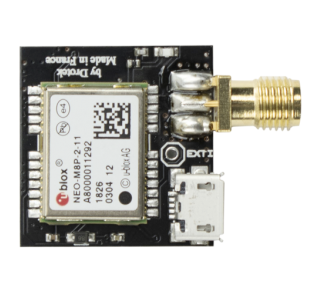
\includegraphics[width=.3\linewidth]{images/gps.png}}\quad
	
	\caption{Các module được sử dụng.}
	\label{3figs}
\end{figure}
\subparagraph{Power:}
Nguồn được sử dụng là nguồn Acquy 12V 7.5Ah, số lượng 2, để tạo ra nguồn 24V cấp cho động cơ.
\subparagraph{Driver}
Do model xe sử dụng 2 động cơ (trái/phải) do đó cần 2 Driver để điều khiển. Board cầu H HI216 có khả năng điều khiển các động cơ có công suất lớn.

\textbf{Các thông số cơ bản:}

 	- Dòng liên tục 15A, dòng đỉnh 20A công suất 600W, tại 25\degree C.
 	
	- Điện áp công suất từ 12V đến 48V.
	
	- Điện áp kích từ 3V3 -> 5V.
	
	- Có cầu chì bảo vệ ngắn mạch.
	
	- Có Led báo nguồn (POW), tín hiệu xung đưa vào (PWM) và và tín hiệu đảo chiều (DIR).
	
	- Board được thiết kế nhỏ gọn với kích thước 52x64x22mm.
	
	- Tần số hoạt động lên tới 100 Khz, sử dụng Opto HCPL-0631 cho tần số hoạt động cao.
	
	- Độ rộng xung 100\%.
\subparagraph{STM32F411}
Kit STM32F411 được dùng để điều động xung, hướng của xe, đọc dữ liệu từ kit GPS, Encoder,...
\subparagraph{RTK GPS}
Được sử dụng để xác định vị trí hiện tại của xe, dựa vào đó để tính toán đưa ra hướng và vận tốc di chuyển tiếp theo của xe.
\subsection{Kết nối các module}
\end{document}